\section{Experimentálne overenie funkčnosti riešenia}

Tato kapitola je venovana overeniu spravnosti implementacie. Boli vykonane nasledujuce styri experimenty, 
ktore mali potvrdit, alebo vyvratit spravnu funkcnost riesenia. 
\begin{enumerate}
 \item \textbf{Prvy test} overil konektivitu a prenos udajov medzi exporterom a mediatorom a nasledne medzi 
 mediatorom a kolektorom.
 \item \textbf{Druhy test} porovnal hodnoty udajov exportovanych mybeem-om s hodnotami ulozenymi v databaze po prechode
 cez Mediator bez sprostredkovatelskeho procesu.
 \item \textbf{Treti test} demonstroval spravnost anonymizacie udajov v podani sprostredkovatelskeho procesu 
 \verb|ExampleProcess|, spominaneho vyssie v navrhu a implementacii
 \item \textbf{Stvrty test} bol tzv. zatazovym testom, overoval stabilitu Mediatora pri dlhodobom behu a pri 
 spracovavani prevadzky s vysokym poctom tokov.
\end{enumerate}

%%%%%

\subsection{Testovacia topológia}

Pri vsetkych testoch bol pouzity virtualizacny nastroj VirtualBox, v ktorom boli vytvorene tri virtualne 
pocitace, zapojene do topologie, ktoru mozno vidiet na Obrazku \ref{o:test_topologia}.
Na vsetkych troch pocitacoch sa pouzival operacny system Ubuntu 12.04 LTS v desktopovej verzii. Na prvom 
pocitaci bol nainstalovany exporter mybeem (verzia 1.1-6 s podporou pre IPFIX Mediator), ktory exportoval 
spravy druhemu pocitacu na UDP port vyhradeny pre IPFIX komunikaciu - \emph{4739}, kde bezal Mediator
verzie 1.0. Ten zase preposielal spravy na treti pocitac (taktiez port \emph{4739}), kde bol spusteny 
kolektor JXColl (verzia 3.9) s funkcnou PostgreSQL databazou. Pocitace boli zapojene v jednej lokalnej 
sieti a vsetky mali pristup na Internet.

\begin{figure}[ht!]
\centering
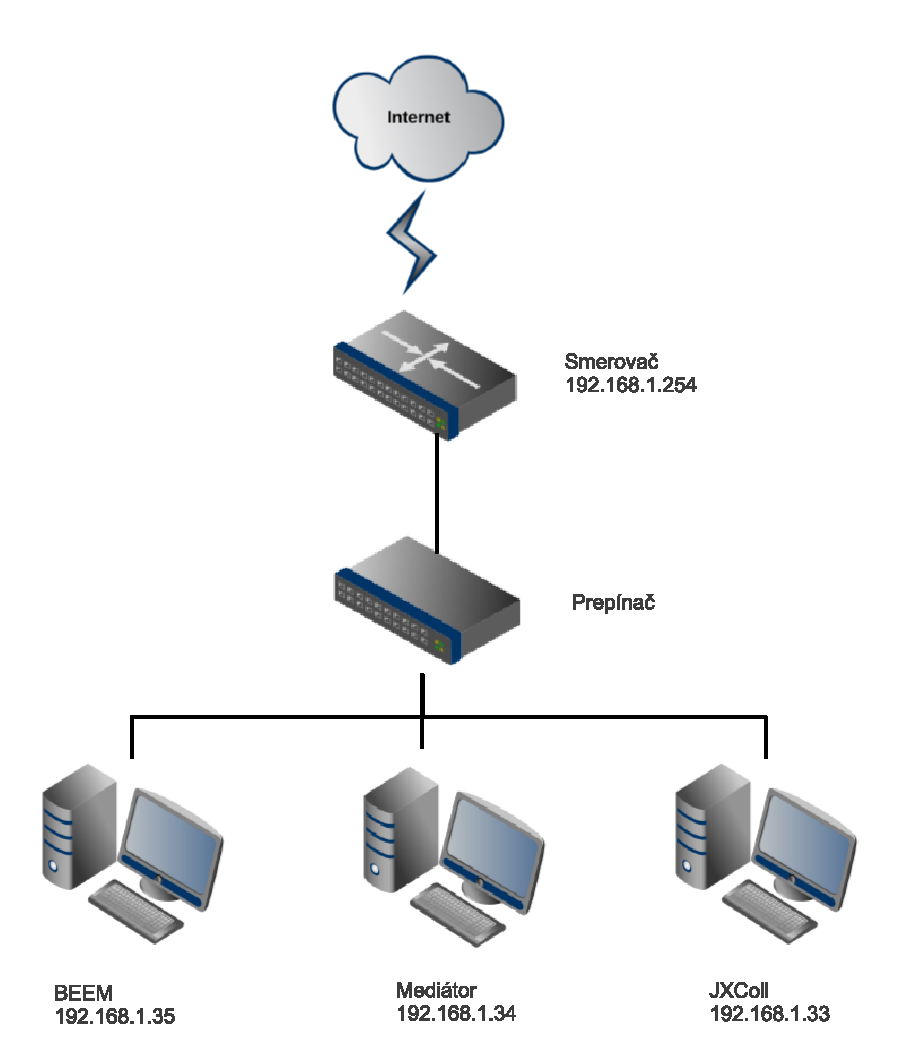
\includegraphics[width=0.8\textwidth]{test_topologia}
\caption{Testovacia topológia}\label{o:test_topologia}
\end{figure}

%%%%%%-----------------

\subsection{Test konektivity}

Prvy experiment overoval zakladnu konektivitu medzi exporterom a kolektorom v pripade, ze je medzi ne 
zaradeny mediator. 

\begin{figure}[ht!]
\centering
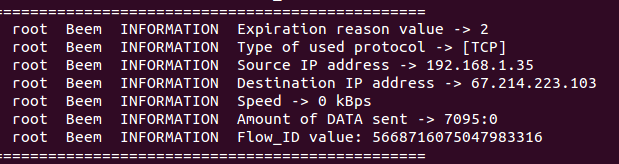
\includegraphics[width=0.9\textwidth]{konektivita_beem}
\caption{Dôkaz konektivity medzi exportérom a Mediátorom - strana exportéra}\label{o:konektivita_beem}
\end{figure}

\begin{figure}[ht!]
\centering
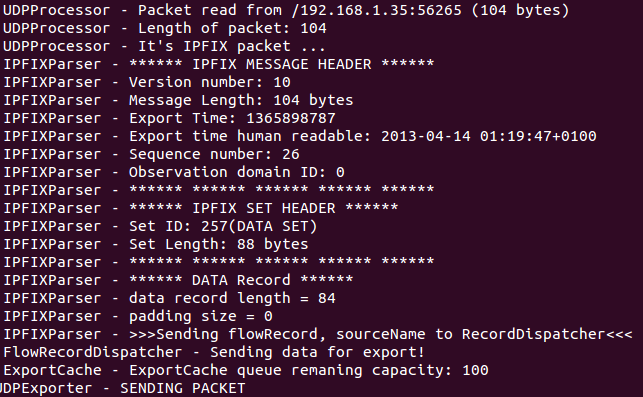
\includegraphics[width=0.9\textwidth]{konektivita_mediator}
\caption{Dôkaz konektivity medzi exportérom a Mediátorom - strana Mediátora}\label{o:konektivita_mediator}
\end{figure}

\subsection{Test spravnej reprezentacie udajov}

\begin{figure}[ht!]
\centering
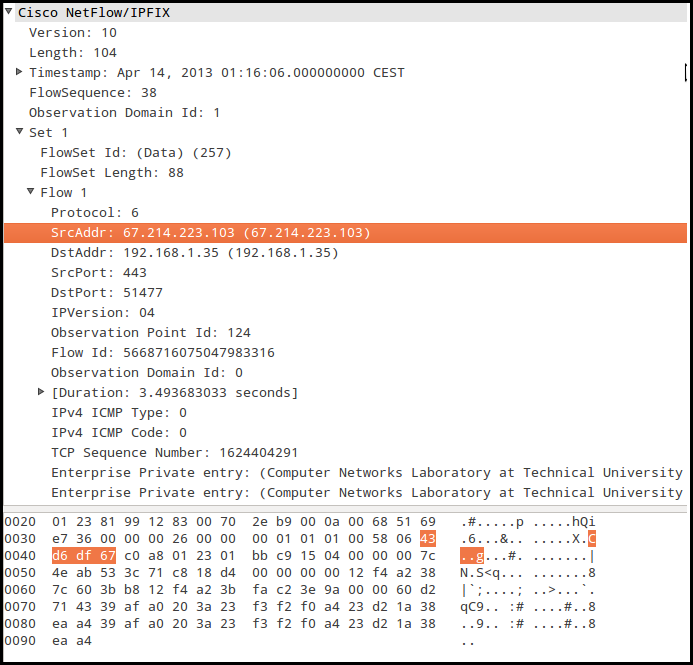
\includegraphics[width=0.9\textwidth]{porovnanie_wireshark}
\caption{Správy odosielané exportérom zachytené programom Wireshark}\label{o:porovnanie_wireshark}
\end{figure}

\begin{figure}[ht!]
\centering
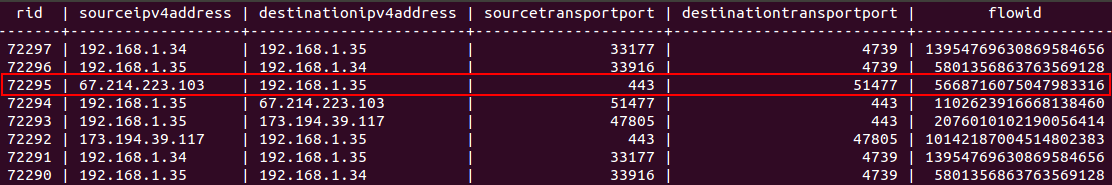
\includegraphics[width=1.0\textwidth]{porovnanie_db}
\caption{Výpis obsahu databázy}\label{o:porovnanie_db}
\end{figure}



\subsection{Test Mediatora s anonymizacnym modulom}
\subsection{Zatazovy test}



